\documentclass{article}
\usepackage[utf8]{inputenc}
\usepackage{geometry}
\geometry{
	paperwidth=35cm,
	paperheight=48cm,
	top=2cm,
	bottom=2cm,
	left=2cm,
	right=2cm,
}
\usepackage{graphicx}
\graphicspath{{../plots/}}
\usepackage[font=Large,labelfont=bf]{caption}
\captionsetup{width=\linewidth}
\usepackage{subcaption}

\begin{document}

	\begin{figure}
		\centering
		\begin{subfigure} {\columnwidth}
				\centering 
				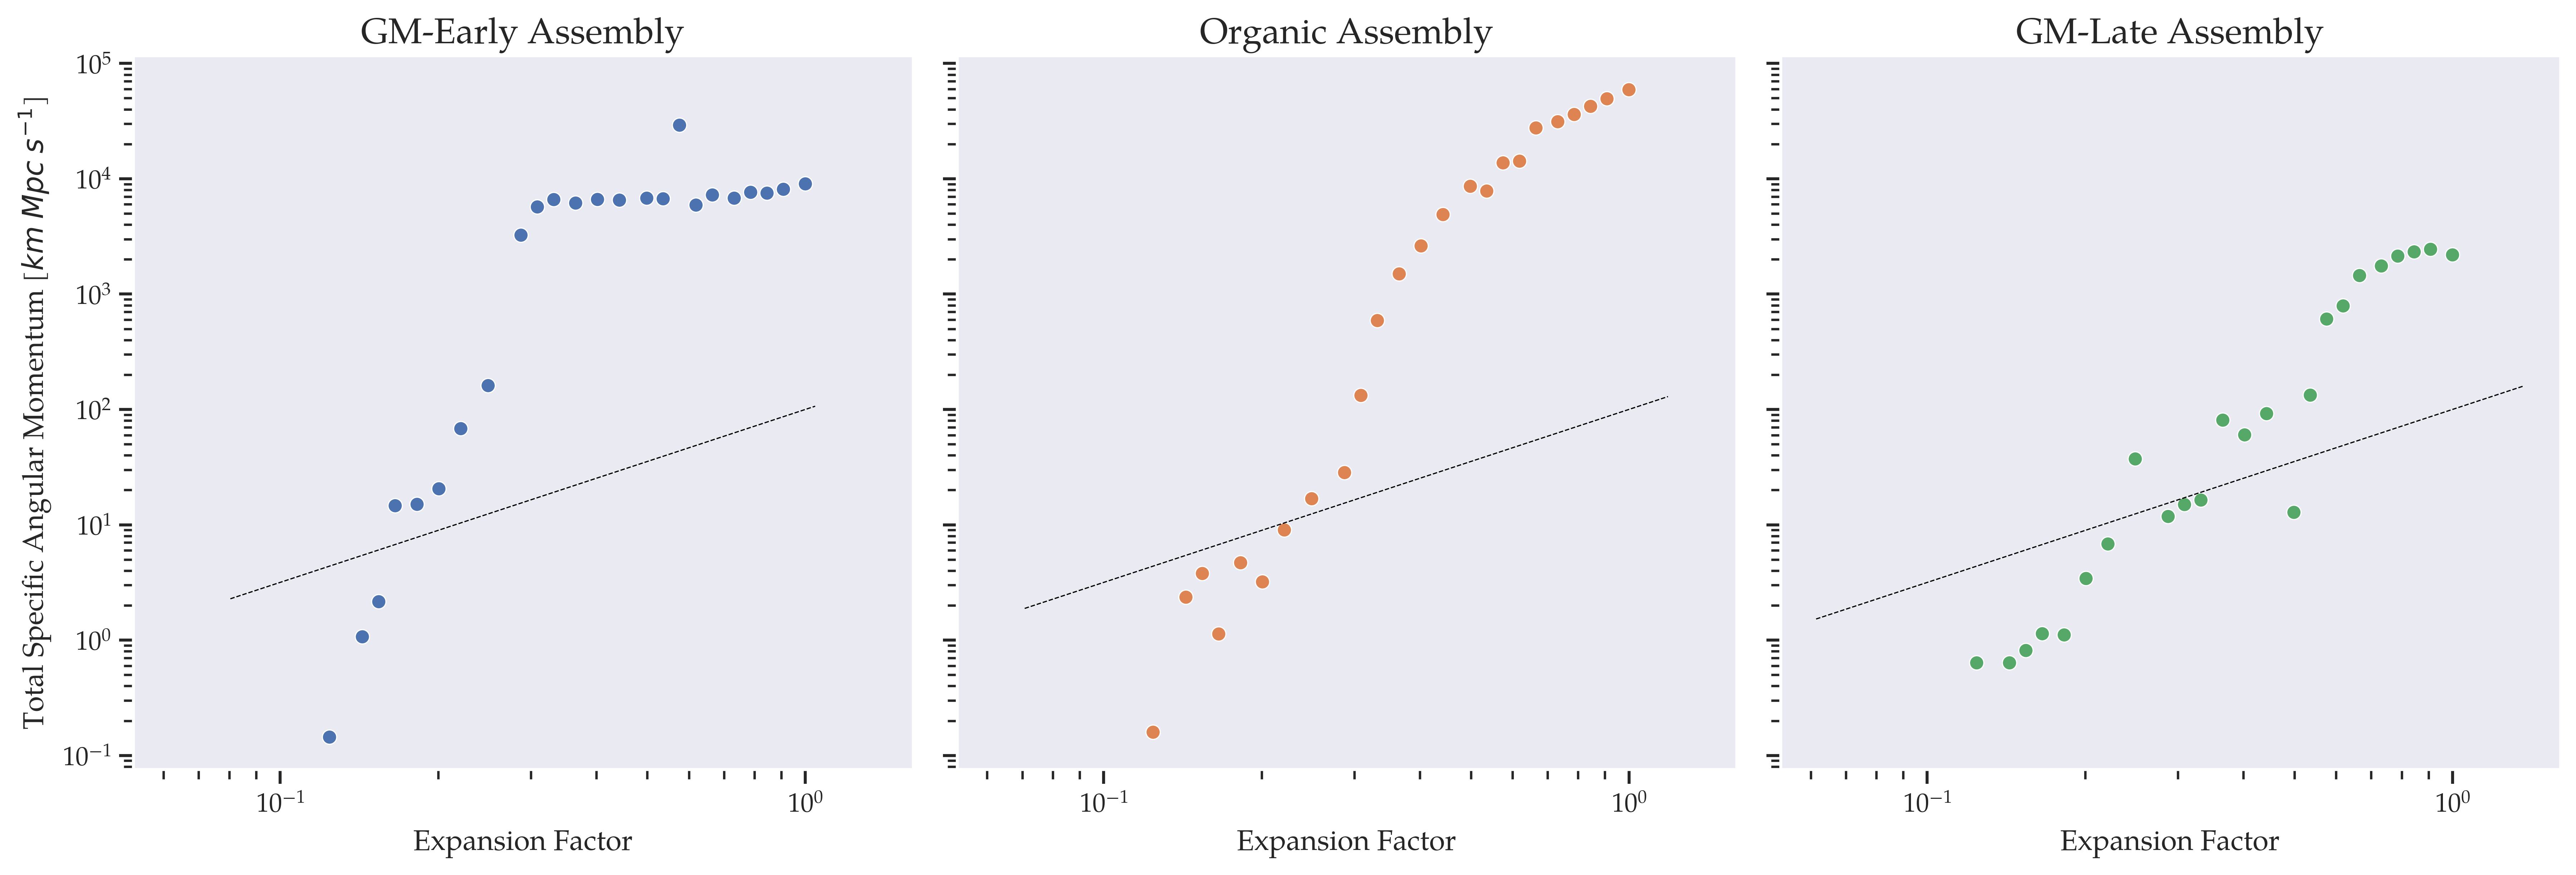
\includegraphics[width=\columnwidth]{../../plots/baryon_cdm/expansion_factor-net_specific_angular_momentum.png}
				\caption{Total specific angular momentum vs expansion factor plot for three assembly modes.}
		\end{subfigure} \\
			% \hfill
			\vspace{1cm}
		\begin{subfigure} {\columnwidth}
				\centering 
				\includegraphics[width=\columnwidth]{../../plots/baryon_cdm/expansion_factor-net_specific_angular_momentum_baryons.png}
				\caption{Total specific angular momentum vs expansion factor plot for \emph{baryon }particles in three assembly modes.}
		\end{subfigure} \\
			\vspace{1cm}
		\begin{subfigure} {\columnwidth}
				\centering 
				\includegraphics[width=\columnwidth]{../../plots/baryon_cdm/expansion_factor-net_specific_angular_momentum_cdm.png}
				\caption{Total specific angular momentum vs expansion factor plot for \emph{cold dark matter} particles in three assembly modes.}
		\end{subfigure}
		\caption{Specific angular momentum vs expansion factor (\(a\)) plots, overlaid by \(a^{3/2}\) dashed black line.}
	\end{figure}

	\clearpage

	\begin{figure}
		\centering
		\begin{subfigure} {\columnwidth}
				\centering 
				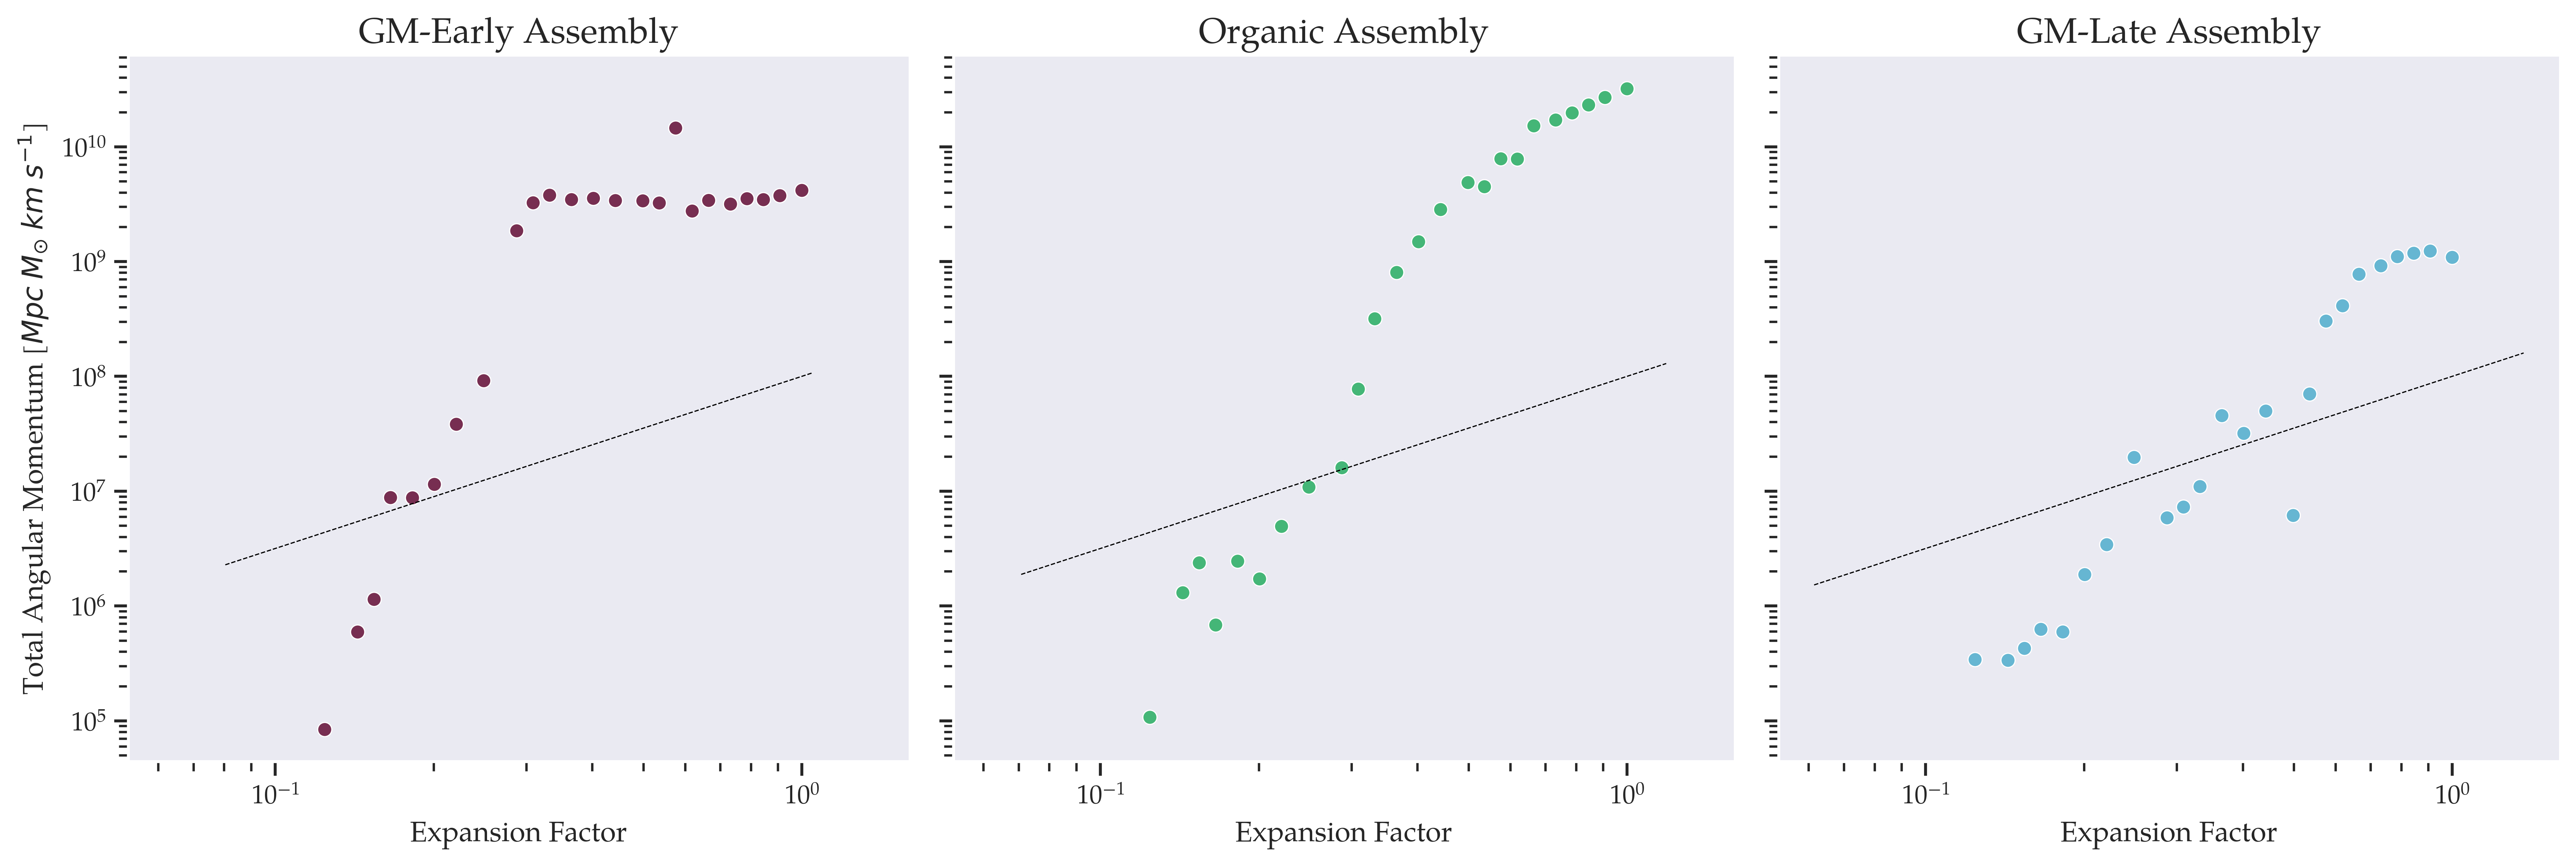
\includegraphics[width=\columnwidth]{../../plots/baryon_cdm/expansion_factor-net_angular_momentum.png}
				\caption{Total angular momentum vs expansion factor plot for three assembly modes.}
		\end{subfigure} \\
			% \hfill
			\vspace{1cm}
		\begin{subfigure} {\columnwidth}
				\centering 
				\includegraphics[width=\columnwidth]{../../plots/baryon_cdm/expansion_factor-net_angular_momentum_baryons.png}
				\caption{Total angular momentum vs expansion factor plot for \emph{baryon }particles in three assembly modes.}
		\end{subfigure} \\
			\vspace{1cm}
		\begin{subfigure} {\columnwidth}
				\centering 
				\includegraphics[width=\columnwidth]{../../plots/baryon_cdm/expansion_factor-net_angular_momentum_cdm.png}
				\caption{Total angular momentum vs expansion factor plot for \emph{cold dark matter} particles in three assembly modes.}
		\end{subfigure}
		\caption{Total angular momentum vs expansion factor (\(a\)) plots, overlaid by \(a^{3/2}\) dashed black line.}
	\end{figure}

	\clearpage 

	\begin{figure}
		\centering
		\begin{subfigure} {\columnwidth}
				\centering 
				\includegraphics[width=\columnwidth]{../../plots/baryon_cdm/expansion_factor-net_specific_angular_momentum_a3by2.png}
				\caption{Total specific angular momentum divided by expansion factor raised to the 3/2 exponent vs expansion factor plot for three assembly modes.}
		\end{subfigure} \\
			% \hfill
			\vspace{1cm}
		\begin{subfigure} {\columnwidth}
				\centering 
				\includegraphics[width=\columnwidth]{../../plots/baryon_cdm/expansion_factor-net_specific_angular_momentum_a3by2_baryons.png}
				\caption{Total specific angular momentum divided by expansion factor raised to the 3/2 exponent vs expansion factor plot for \emph{baryon} particles in three assembly modes.}
		\end{subfigure} \\
			\vspace{1cm}
		\begin{subfigure} {\columnwidth}
				\centering 
				\includegraphics[width=\columnwidth]{../../plots/baryon_cdm/expansion_factor-net_specific_angular_momentum_a3by2_cdm.png}
				\caption{Total specific angular momentum divided by expansion factor raised to the 3/2 exponent vs expansion factor plot for \emph{cold dark matter} particles in three assembly modes.}
		\end{subfigure}
		\caption{Specific angular momentum divided by expansion factor raised to the 3/2 exponent vs expansion factor (\(a\)) plots, overlaid by \(a^{3/2}\) dashed black line.}
	\end{figure}

\end{document}